\section{Jagttidsbekendtgørelsen}

\begin{frame}
  \vspace{3em}
  \begin{center}
    {\LARGE \textbf{Jagttidsbekendtgørelsen}}
    \vspace{2em}
    \\ Bekendtgørelse om jagttid for visse pattedyr og fugle m.v.
\par

{\normalsize \href{https://www.retsinformation.dk/eli/lta/2024/470}{BEK nr 470 af 17/05/2024 \\
§§ 1-5 | Bilag 1}}
\vspace{1em}
\par
  \end{center}
\end{frame}

\begin{frame}{Jagttidsregler – Simpel oversigt}
  \begin{itemize}
    \item \textbf{Generelle jagttider (§ 1)}  
      Se \textbf{Bilag 1} – baseret på EU-direktiver + dansk jagtlov.

    \item \textbf{Lokale jagttider (§ 2)}  
      Fraviger generelle tider i visse områder → \textbf{Bilag 2–4} (ændringer) + \textbf{Bilag 5–28} (kort).  
      Dyrehaver følger generelle tider.

    \item \textbf{Tidsrum for jagt (§ 3)}  
      Hovedregel: Kun \alert{solopgang til solnedgang}.  
      \small Undtagelser:
      \begin{itemize}
        \item Ænder \& gæs: 1½ t før solopgang → 1½ t efter solnedgang
        \item Kronvildt: Kan have anden tid (Bilag 3)
        \item Husskade, gråkrage, sortkrage: 1 t før solopgang → solnedgang
      \end{itemize}
  \end{itemize}
\end{frame}

\begin{frame}{Andre vigtige regler}
  \begin{itemize}
    \item \textbf{Overdragelse af jagtret (§ 4)}  
      Ande-/vadefugle + vandhøns (undt. skovsneppe \& opdrættede gråænder):  
      Kan ikke overdrages kortere end \textbf{1 år}.

    \item \textbf{Dispensation (§ 5)}  
      Miljøstyrelsen kan give tilladelse til fravigelse fra §§ 1–3.  
      \textbf{Afgørelser kan ikke påklages}.

    \vspace{1em}
  \end{itemize}
\end{frame}
\begin{frame}{Generelle jagttider (Bilag 1 til Jagttidsbekendtgørelsen)}
    \centering
    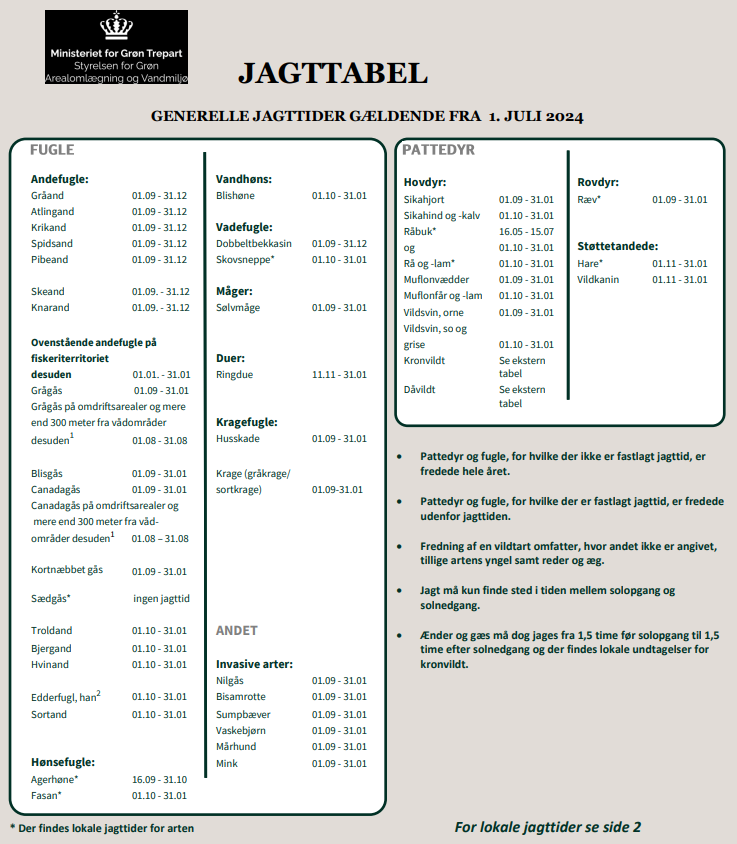
\includegraphics[width=0.42\textwidth]{Billeder/Andet/jagttider.png}
\end{frame}